\documentclass[tikz, border=5mm]{standalone}

\begin{document}
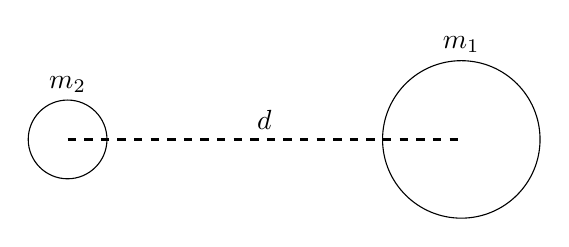
\begin{tikzpicture}
  % Définir une couleur pour le schéma
  \definecolor{mycolor}{RGB}{0,0,0}

  % Dessiner le cercle (la terre)
  \draw[mycolor] (0,0) circle (0.5cm);
  \node[mycolor] at (0,0.7) (moon) {$m_{2}$};

  % Dessiner la lune
  \draw[mycolor] (5,0) circle (1cm);
  \node[mycolor] at (5,1.2) (moon) {$m_{1}$};




  % Dessiner la ligne pointillée de la terre à la lune
  \draw[mycolor, dashed, thick] (0,0) -- (5,0);


  % Ajouter les étiquettes R0 et R
  \node[mycolor, above] at (2.5,0) {$d$};
\end{tikzpicture}
\end{document}
